\chapter{Estatística bivariada}

\begin{myquoting}{Sherlock Holmes em 'Um estudo em Vermelho'}
	
	Como em outras artes,  a ciência da dedução e análise é uma que não pode ser adquirida por um longo e paciente estudo, nem é a vida longa o suficiente para permitir qualquer mortal se ater a mais alta perfeição nela.  
\end{myquoting}

\section{Introdução}

Na análise de bancos de dados geralmente se torna necessário comparar duas populações diferentes. Em um depósito mineral, por exemplo, podemos ter diversas variáveis presentes. Em alguns casos a relação entre elas pode ser um indício dos fenômenos genéticos de formação das rochas. Em outros casos apenas estamos interessados em como uma informação secundária pode estar relacionada com uma primária de interesse. Seria proveitoso para nós, por exemplo, traçar um modelo que definisse a chance de obter uma amostra com certo teor em contrapartida de outra amostra com o teor de uma variável diferente. Em um depósito vulcanogênico sulfetado podemos estar interessados em prever a quantidade de um elemento metálico a partir do enxofre da rocha encaixante. Enfim, toda a informação que relaciona duas variáveis pode ser descrita pela estatística bivariada.  

Diferentemente da estatística univariada, a comparação de histogramas de variáveis diferentes não é uma alternativa interessante sobre o ponto de vista prático. É muito difícil determinar a relação entre duas amostras simplesmente pelas suas proporções individuais. Para isso definimos algumas ferramentas que facilitam ao modelador entender a relação entre duas variáveis distintas visualmente e numericamente. 

As seções que se prosseguem mostrarão algumas das ferramentas utilizadas para se caracterizar distribuições bivariadas. Inicialmente apresentamos as \textbf{ferramentas gráficas} mais utilizadas e depois algumas \textbf{estatísticas pontuais} utilizadas. 

\section{Probabilidade condicional e Esperança condicional} 

\subsection{Probabilidades condicionais e conjuntas}

Probabilidades não são nada além de métricas de conjuntos, proporções de acordo um espaço amostral ($\Omega$). Estas proporções podem tomar diferentes características quando analisamos não apenas um conjunto individual, mas a interação entre eles. Muitas vezes não estamos interessados em determinar as probabilidades ou frequências individuais de uma variável aleatória. É interessante, por exemplo, determinar combinações entre variáveis e suas possíveis relações. E se desejarmos saber qual é a frequência de um minério e que seu conteúdo tenha um determinado valor de impureza? Se denotarmos $X$ como o evento de ser minério, e $Y$, a variável que denota seu limite de impurezas, podemos denotar a probabilidade de $P(X,Y)$ como sendo a probabilidade de que \textit{"Um material seja minério e apresente impurezas acima do limite desejado"}. A forma mais simples de se entender probabilidades é de acordo com um diagrama de Venn, como na figura \ref{disjuntos}

\FloatBarrier
\begin{figure}[!htpb]
	\centering
	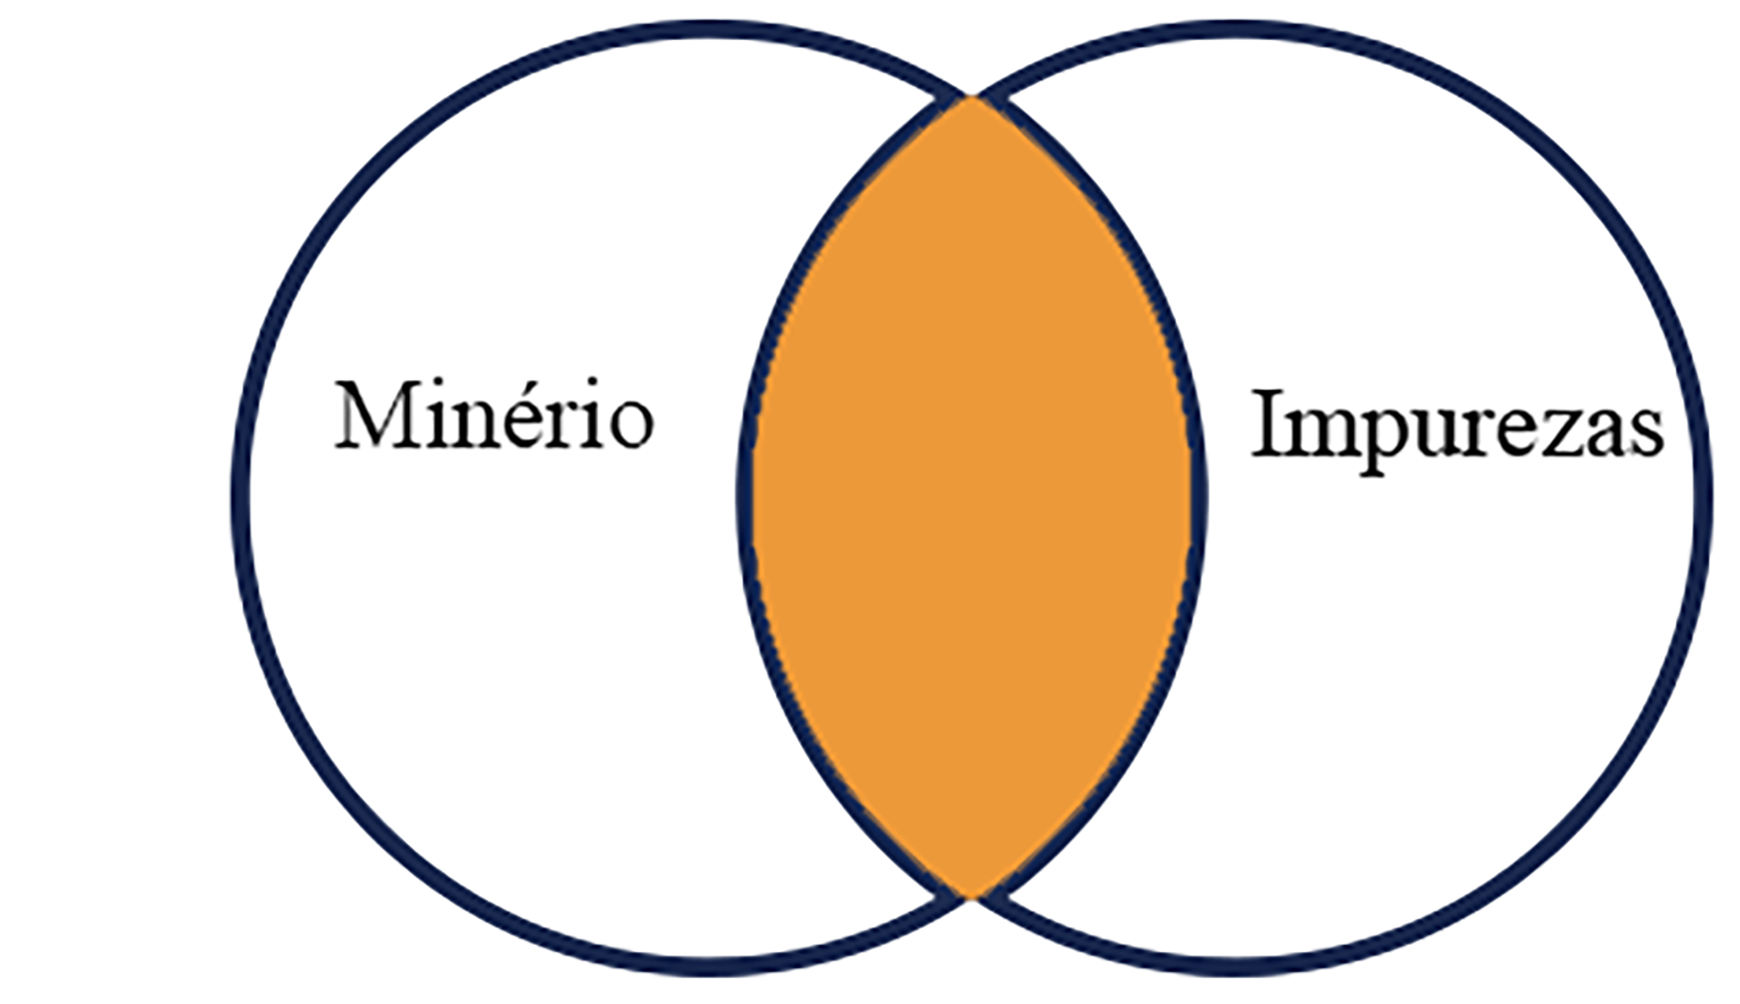
\includegraphics[scale=0.4]{./Capitulo_3/DISJUNTO.png}	
	\caption{Demonstração de eventos disjuntos entre a variável minério e impureza a partir de um diagrama de Venn. Nota-se a área laranja como sendo a interseção dos eventos representado pela probabilidade $P(X,Y)$ }
	\label{disjuntos}
\end{figure}
\FloatBarrier

Observe a tabela \ref{tabela_impureza}. Notamos na coluna três o número de vezes que o minério considerado possui uma impureza maior ou igual a 0,005. Neste caso sabemos que há 2 valores em cinco em que isso ocorre. Logo a probabilidade conjunta é P(Minerio) $\bigcap$ P(Impureza $\geq$  0.005) = 2/5 = 40\%

\FloatBarrier
\begin{table}[!htpb]
	\centering
	\caption{Tabela da relação entre um dado minério e uma impureza}
	\label{tabela_impureza}
	\begin{tabular}{ccc}
		\toprule
		Minério & Impureza & Minério $\bigcap$ (Impureza \textgreater=0,005) \\ \midrule
		Sim     & 0,005    & 1                                                           \\
		Não     & 0,007    & 0                                                           \\
		Não     & 0,008    & 0                                                           \\
		Sim     & 0,006    & 1                                                           \\
		Sim     & 0,003    & 0                                                           \\ \bottomrule
	\end{tabular}
\end{table} 
\FloatBarrier

Em alguns casos também é importante determinar a conjunção entre os eventos, ou a probabilidade de $P(X \vee Y)$. Neste caso queremos determinar \textit{"Um material seja minério ou apresente impurezas acima do limite desejado"}. Note que a conjunção 'ou' é um conectivo lógico muitas vezes díspare do seu uso corriqueiro no português. Ser um ou outro na verdade não é uma escolha entre um dos elementos, mas uma soma dos eventos. A representação da conjunção pode ser vista na figura \ref{conjuncao}.

\FloatBarrier
\begin{figure}[!htpb]
	\centering
	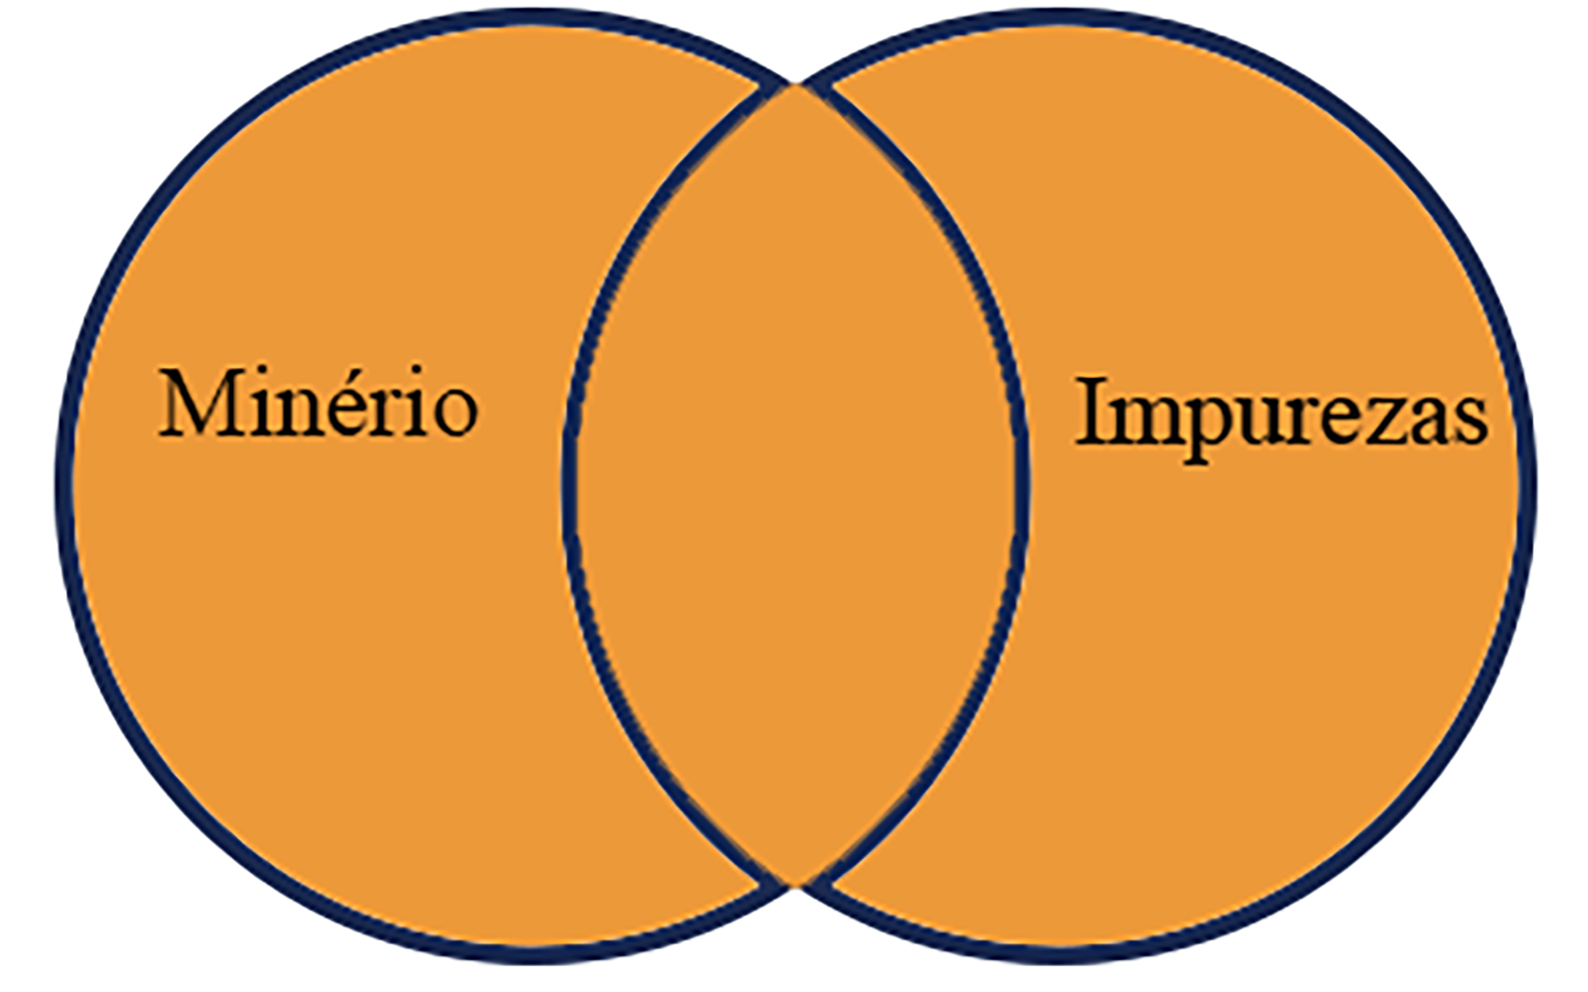
\includegraphics[scale=0.4]{./Capitulo_3/conjucao.png}	
	\caption{Demonstração da conjunção de eventos entre a variável minério e impureza a partir de um diagrama de Venn. Nota-se a área laranja como sendo a interseção dos eventos representado pela probabilidade $P(X\vee Y)$ }
	\label{conjuncao}
\end{figure}
\FloatBarrier

Estas relações lógicas envolvem o conhecimento entre os eventos independentemente. Conhecer $P(X,Y)$ é examente o mesmo que conhecer $P(B,A)$. Em alguns casos devemos entender o conceito de dependência na estatística, expresso pela probabilidade condicional. Neste caso queremos saber \textit{"dado que um material apresente impurezas, qual é sua probabilidade de ser minério"}. Esta é uma afirmação muito diferente da obtida nos outros casos, pois para sabermos se algo é minério, precisamos saber antes se ele contém impurezas. A probabilidade condicional $P(X|Y)$ pode ser demonstrada pela  figura \ref{disjuntos2} como a relação da área laranja pela área hachurada.

\FloatBarrier
\begin{figure}[!htpb]
	\centering
	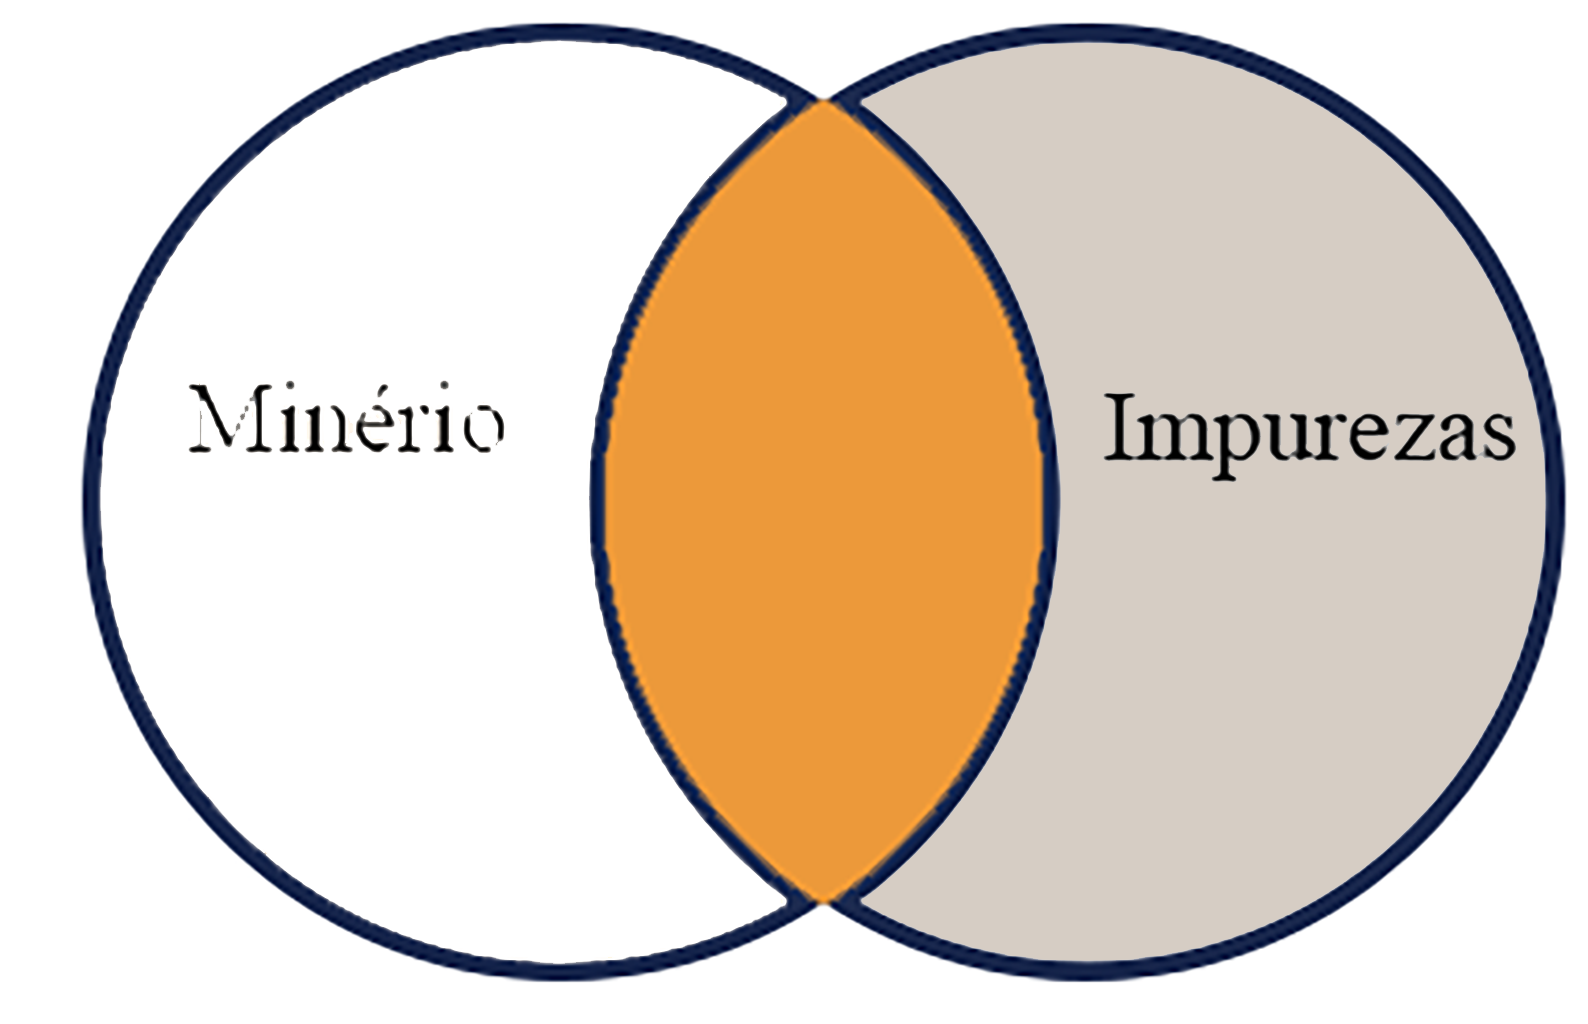
\includegraphics[scale=0.4]{./Capitulo_3/DISJUNTO_2.png}	
	\caption{Demonstração da probabilidade condicional entre a variável minério e impureza a partir de um diagrama de Venn.Nota-se a área laranja como sendo a interseção dos eventos disjuntos. A probabilidade condicional é a relação entre a área laranja pela área hachurada. }
	\label{disjuntos2}
\end{figure} 
\FloatBarrier

Esta relação também é chamada de teorema de Bayes, e envolve a equação \eqref{Bayes}

\begin{equation}\label{Bayes}
P(X|Y) = \frac{P(X,Y)}{P(Y)}
\end{equation}

\begin{proposition}
	\textit{As probabilidades condicionais expressam um importante conceito na geoestatística, a dependência entre variáveis aleatórias. Quando estudamos fenômenos espaciais, os valores obtidos em um suporte específico $x_{1}$ são muito mais dependentes de $x_{2}$ do que $x_{3}$, se a distância de $\left\{ x_{1},x_{2} \right\}$ for menor que a distância de $\left\{ x_{1},x_{3} \right\} $} 
\end{proposition}

\subsection{Esperança condicional}

A partir da definição de probabilidade condicional também é possível determinar a esperança condicional. Ela nada mais é que o valor médio obtido e uma variável $Y$ dado que a variável $X$ assuma um valor específico $x$. Por exemplo, podemos determinar qual é a probabilidade do material ser contaminado $Y$, dado que a presença de um litotipo $X$ seja $x =\{itabirito\}$, de acordo com a equação \eqref{pcond}.  

\begin{equation}\label{pcond}
E(Y|X=x) = \sum_{y \in Y} y P(Y =y|X=x)
\end{equation}

Considere que $Y$ seja uma variável binária tal que assuma o valor $0$ para o elemento contaminado, e valor $1$ para não contaminado. A variável $X$ pode assumir os valores de itabirito e calcário no problema. Analisando a tabela \ref{tabela_condic} podemos determinar as probabilidades de acordo com os respectivos valores apresentados. 


\FloatBarrier
\begin{table}[!htpb]
	\centering
	\caption{Tabela da relação entre um minério contaminado e litotipo}
	\label{tabela_condic}
	\begin{tabular}{cccc}
		\toprule
		Y & X & (Y=0| X=itabirito ) & (Y=1| X=itabirito)  \\ \midrule
		contaminado         & itabirito    & 1    &0                                                       \\
		descontaminado     & calcário     & 0    &0                                                       \\
		descontaminado     & calcário     & 0    &0                                                       \\
		contaminado         & itabirito    & 1    &0                                                       \\
		descontaminado     & itabirito    & 0    &1                                                       \\ \bottomrule
		P(Y=y|X=x) 		&              &2/3   &1/3													   \\ \bottomrule
	\end{tabular}
\end{table} 
\FloatBarrier

O valor esperado condicional pode ser obtido a partir da tabela pode ser calculado por \eqref{result}

\begin{equation}\label{result}
E(Y|X=itabirito) = 2/3.0 + 1/3.1 = 1/3
\end{equation}

No caso de variáveis reais, aos quais as probabilidades não são explícitas diretamente, opta pelo uso de estatísticas intervalares. Neste caso desejamos obter $E(Y| x_{1}<X<x_{2})$. Podemos obter, por exemplo, o valor da recuperação metalúrgica de carvão, dado que os valores de enxofre estejam entre $5\%$ e $6\%$, por exemplo.  O valor da esperança condicional considerando uma distribuição contínua das variáveis $X$ e $Y$ pode ser expressa pela equação \eqref{condici2}

 \begin{equation}\label{condici2}
 E(Y|X) = \int_{-\infty}^{-\infty} y f_{Y|X}(y,x) dy
 \end{equation}

Onde $f_{Y|X}(y,x)$ representa a função de densidade de probabilidade condicional. A figura \ref{histcond} apresenta como calcular estatísticas condicionais considerando estatísticas intervalres. O histograma, ou a distribuição dos dados são consideradas dentro dos limites específicos $x_{1}<X<x_{2}$, para um determinado tamanho da classe. 

\FloatBarrier
\begin{figure}[!htpb]
	\centering
	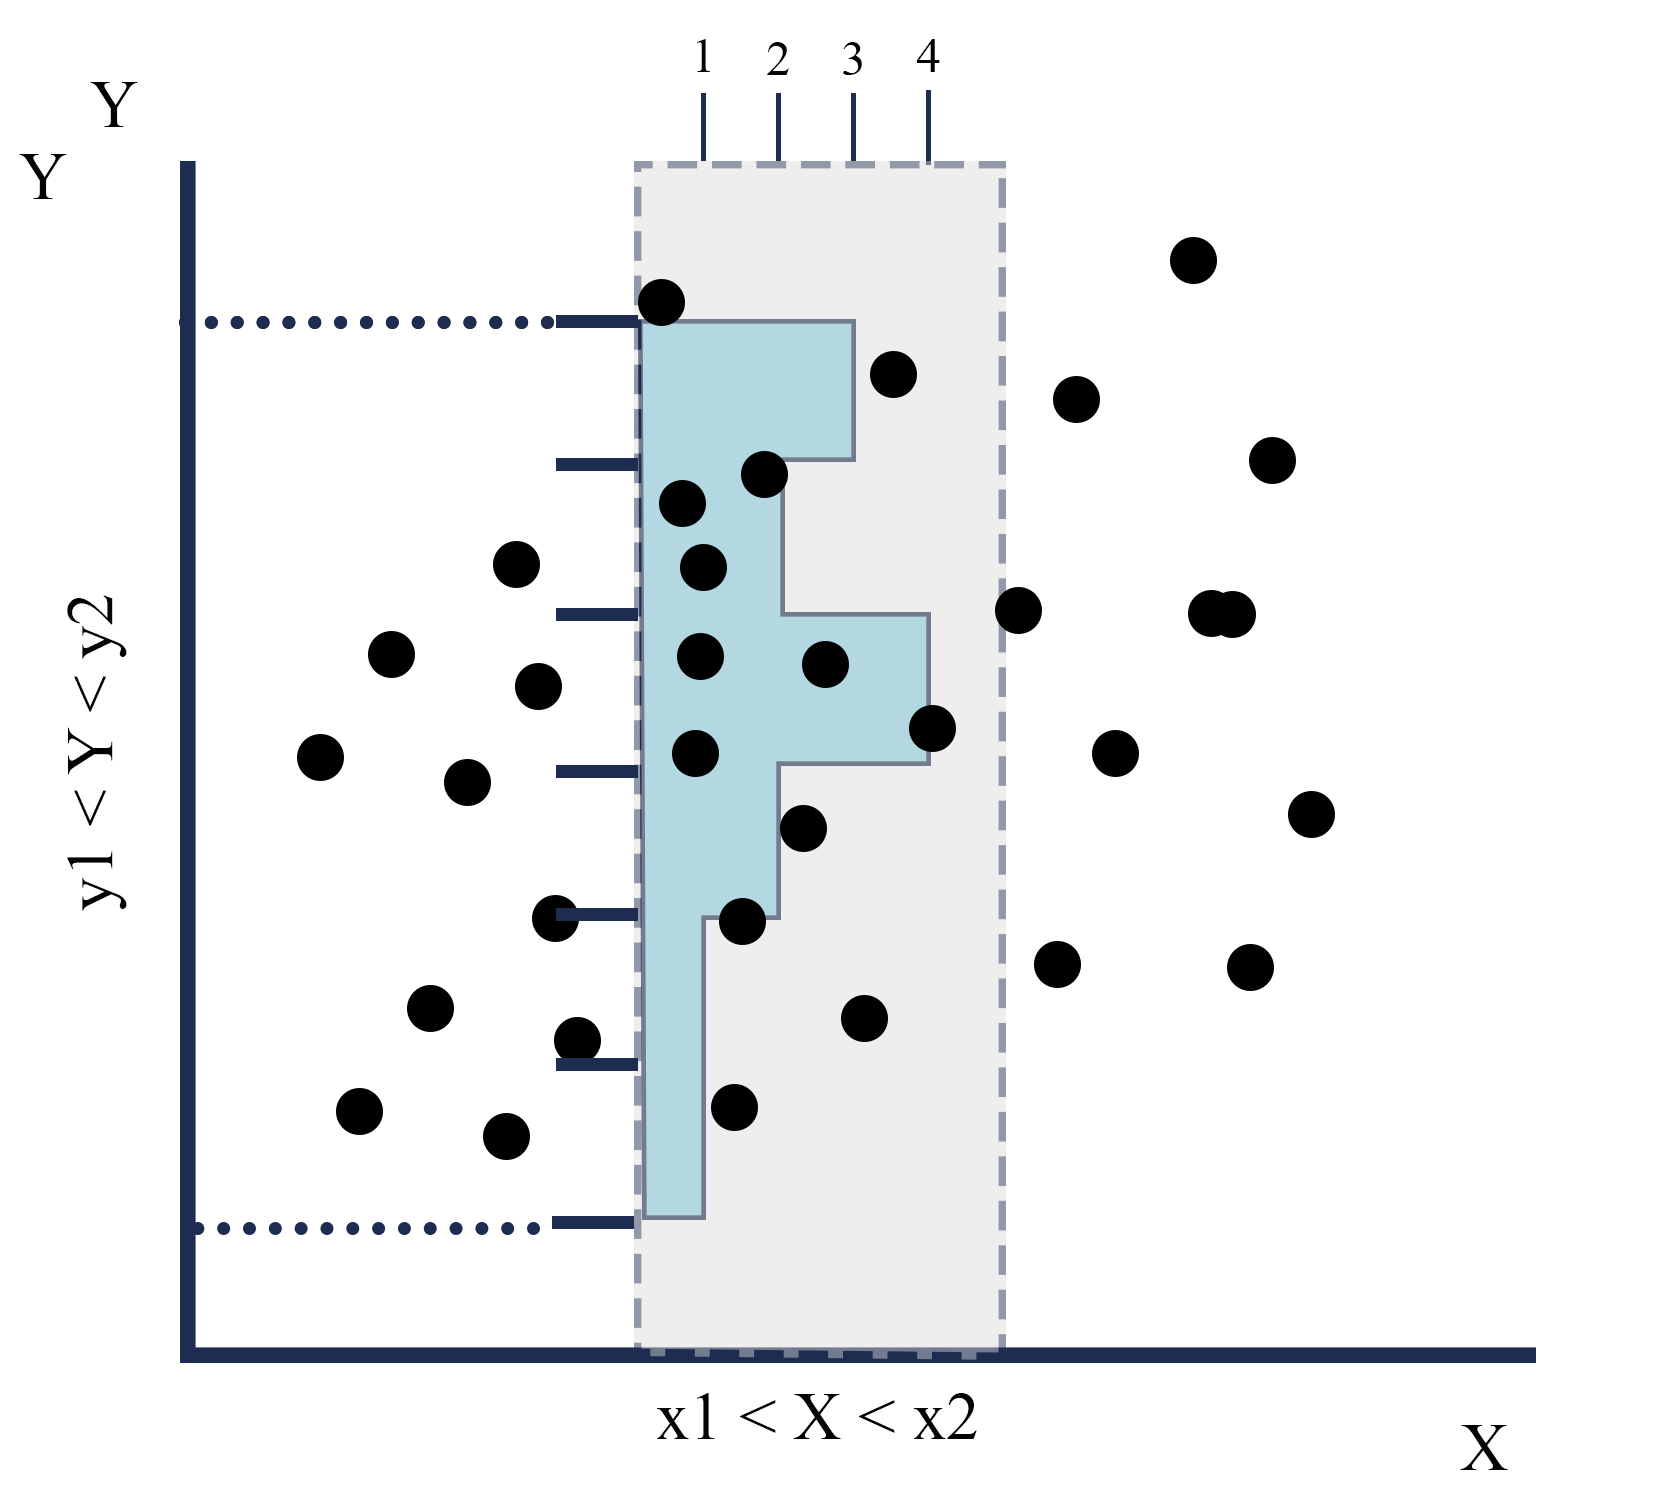
\includegraphics[scale=0.8]{./Capitulo_3/hist_cond.png}	
	\caption{Demonstração do histograma condicional considerando um intervalo de $x_{1}<X<x_{2}$ e $y_{1}<Y<y_{2}$. Podemos considerar  }
	\label{histcond}
\end{figure} 
\FloatBarrier

\section{Ferramentas gráficas}

\subsection{Gráfico Q-Q plot}

O gráfico q-q plot é uma ferramenta para uma primeira análise de diferentes distribuições de variáveis aleatórias. Para cada par conjugado são plotados os quantis de uma variável juntamente com outra. Variáveis que possuam distribuição semelhante tendem a apresentar um comportamento segundo uma reta $y=x$, de inclinação $45^{\circ}$. 

Quando as variáveis apresentam a mesma forma, mas deslocamentos diferentes, ou seja, médias diferenciadas, o gráfico q-q plot apresenta o mesmo formato de uma reta, mas um deslocamento em sua abcissa. Quando as distribuições possuem formas semelhantes, mas variâncias diferentes, a distribuição tende a ter uma inclinação diferente. No entanto, quando distribuições possuem assimetrias e formas diferentes, o gráfico q-q plot tende a produzir uma convexidade diferente. A Figura \ref{QQplot} demonstra o gráfico q-q plot das variáveis Cobalto e Cádmio.

\FloatBarrier
\begin{figure}[!htb]
	\centering
	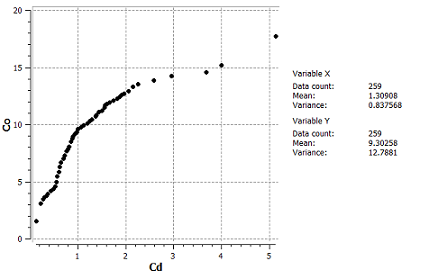
\includegraphics[width=\textwidth]{./Capitulo_3/qq-plot.png}	
	\caption{Gráfico QQ-Plot de Cobalto e Cádmio. Nota-se uma curvatura característica demonstrando pequena correspondência entre as duas populações. Cada ponto representa o mesmo quantil para cada variável }
	\label{QQplot}
\end{figure}
\FloatBarrier

Nota-se na figura que o formato do q-q plot é convexo, demonstrando que as distribuições de dados seguem leis diferenciadas. A figura \ref{histograms} demonstra a comparação entre os histogramas. 

\FloatBarrier
\begin{figure}[!htb]
	\centering
	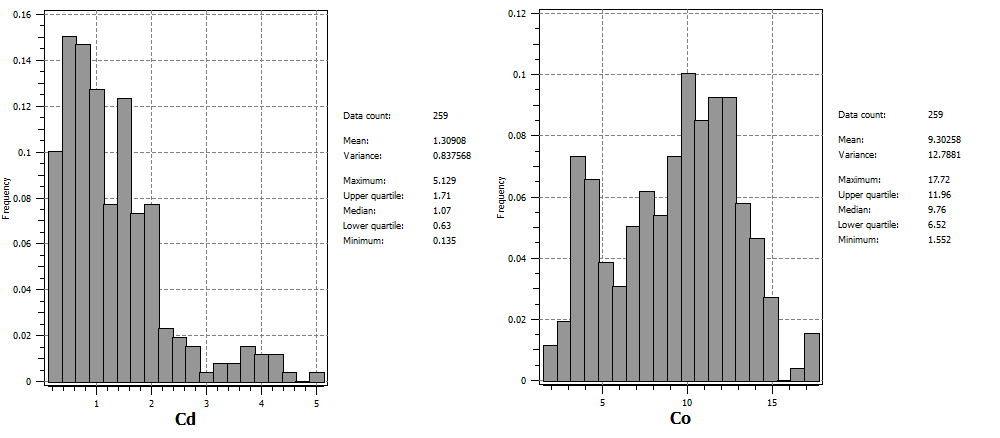
\includegraphics[width=\textwidth]{./Capitulo_3/histograms.png}	
	\caption{Diferenças entre os histogramas de Cádmio e Cobalto}
	\label{histograms}
\end{figure}
\FloatBarrier

\begin{proposition}
	\textit{O gráfico q-q plot é uma alternativa para comparar distribuições de variáveis diferentes. A utilização da ferramenta, deve ser no entanto, utilizada com sabedoria. Valores outliers podem prejudicar a comparação entre as distribuições, o que não significa que possam ser identificadas como possíveis distribuições semelhantes.}
\end{proposition}

Gráficos q-q plot podem ser utilizados não apenas entre amostras, mas também com uma combinação de uma variável amostrada e os quantis teóricos de uma distribuição. Uma das formas de se averiguar a normalidade de uma distribuição é comparar as amostras padronizadas $Z_{pad} = (Z - \bar{x})/S$ com uma variável gaussiana padrão $\phi(0,1)$. A figura \ref{QQplot_adjust} demonstra 

\FloatBarrier
\begin{figure}[!htb]
	\centering
	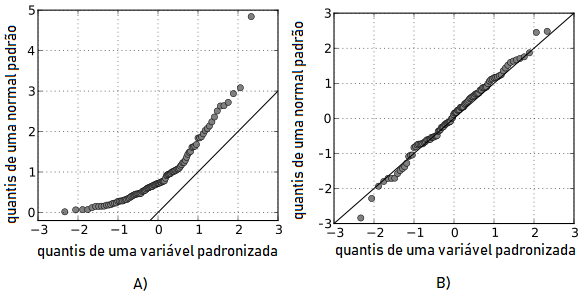
\includegraphics[scale=0.6]{./Capitulo_3/q_q_fit.png}	
	\caption{Gráfico da utilização do q-q plot para ajuste de uma distribuição. Quantis de uma amostra padronizada comparadas com quantil de uma distribuição gaussiana padrão. A) Mal ajuste. B) Bom ajuste }
	\label{QQplot_adjust}
\end{figure}
\FloatBarrier

\subsection{Gráfico p-p plot}

Semelhante ao gráfico q-q plot temos o gráfico p-p plot. O gráfico de probabilidades implica nos pares conjugados que indicam a mesma probabilidade $\left(Pr(Z<z),Pr(Y<z)\right) \forall z \in Z,Y $. A figura \ref{ppplot} demonstra o gráfico da variável Cobre pela de Cromo. 

\FloatBarrier
\begin{figure}[!htb]
	\centering
	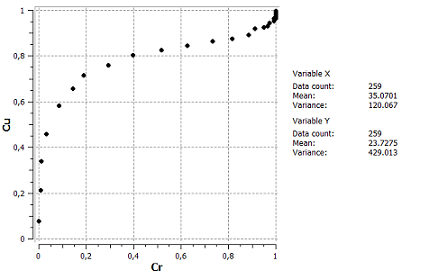
\includegraphics[width=\textwidth]{./Capitulo_3/pp-plot.png}	
	\caption{Gráfico PP-Plot de Cobre e Cromo. Nota-se uma curvatura característica demonstrando pouca correspondência entre as duas populações. Cada ponto representa o percentual acumulado para o mesmo valor da variável aleatória }
	\label{ppplot}
\end{figure} 
\FloatBarrier

Podemos notar que as diferenças demonstradas no gráfico p-p plot se reproduzem nas diferenças entre os hitogramas de cobre e cromo na figura \ref{histograms2}

\FloatBarrier
\begin{figure}[!htb]
	\centering
	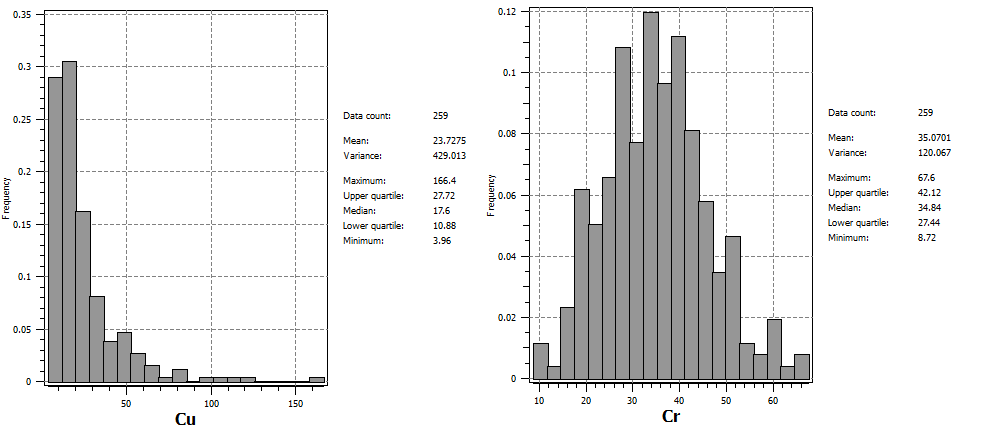
\includegraphics[width=\textwidth]{./Capitulo_3/histograms2.png}	
	\caption{Diferenças entre os histogramas de Cobre e Cromo}
	\label{histograms2}
\end{figure}
\FloatBarrier

A análise do gráfico é feita de forma semelhante ao QQ-plot, no entanto, este gráfico é muito mais sensível à mudança de escala das variáveis. Ele é mais vantajoso quando a ordem de grandeza das variáveis analisadas for semelhante. Neste caso estamos comparando a relação de percentuais acumulados diferentes para o mesmo valor da variável aleatória. 

\subsection{Gráfico de dispersão}
  
O gráfico de dispersão apresenta dados de duas variáveis dispostos nos eixos cartesianos. Temos uma variável \textbf{preditora} (X) e uma variável \textbf{resposta} (Y). Os pares conjugados $(x_{i}, y_{i}) \in X,Y$ representam pontos em um plano cartesiano.

\begin{proposition}
	\textit{Uma das primeiras utilizações da regressão linear foi no estudo da importância de tendências entre gerações. Durante o período de 1893-1898, E. S. Pearson organizou uma coleção de n=1375 alturas de mães do reino Unido abaixo de 65 anos e uma de suas filhas acima de 18. O interesse era computar o tamanho das mães (Mheight) com o tamanho das filhas (Dheight) como preditor. Se todas as mães possuirem tamanho igual suas filhas, os dados estarão dispostos em uma reta de inclinação $45^{circ}$. A linearidade proposta pela dispersão identifica que mães mais altas geralmente possuem filhas mais altas.} - \cite{weisberg2005applied}
\end{proposition}

Para a utilização do gráfico os dados devem estar colocados. Isso significa que a amostra 1 deve ter a mesma origem da amostra 2, ou o mesmo suporte. Logo só podemos realizar um gráfico de dispersão com vetores de amostras do mesmo tamanho. 

Caso a amostragem apresente dados inválidos para uma variável devemos utilizar um filtro para separar apenas os dados colocados. Existem técnicas estatísticas que permitem o tratamento de dados perdidos ou inexistentes, mas nada substitui a amostra em termos de informação sobre o objeto de estudo. A figura \eqref{scatter} demonstra um gráfico de dispersão entre a variável cromo e cobalto.
  
\begin{figure}[H]
  	\centering
  	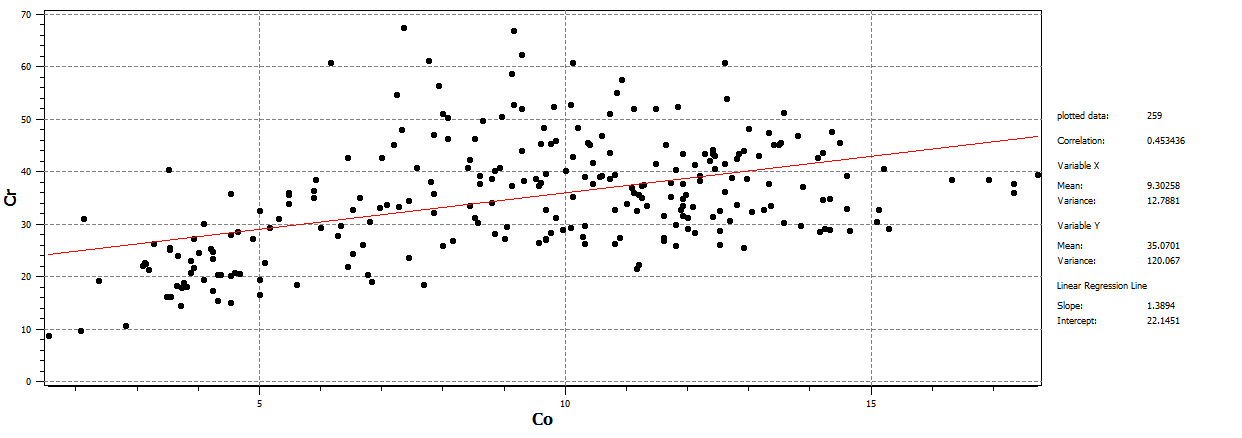
\includegraphics[width=\textwidth]{./Capitulo_3/scatter.png}	
  	\caption{Gráfico de dispersão da variável Cromo e Cobalto. Nota-se dependência linear positiva entre as variáveis. }
  	\label{scatter}
\end{figure} 
   
Nota-se pela figura que as variáveis possuem \textbf{dependência linear positiva} entre a variável Cromo e Cobalto. Isso significa que amostras com valor grande de cromo podem apresentar valores grandes de cobalto. O contrário também pode acontecer, alguns minerais como quartzo e piroxênio são inversamente proporcionais em rochas magmáticas. À medida em que se aumenta o teor de quartzo tende-se a reduzir o teor de piroxênio na amostra de rocha. Neste caso possuímos uma \textbf{dependência linear negativa} 

A Figura \ref{correlacao_linear} demonstra os tipos de correlação lineares possíveis. Em \ref{correlacao_linear} -a temos a correlação linear positiva em que o aumento da variável X aumenta o valor de Y, em \ref{correlacao_linear} -b temos a correlação linear negativa em que o aumento do valor X tende a diminuir o valor de Y e em \ref{correlacao_linear} -c temos um caso de independência entre as variáveis, tal que o aumento da variável X não altera o valor da variável Y. 

\begin{figure}[H]
	\centering
	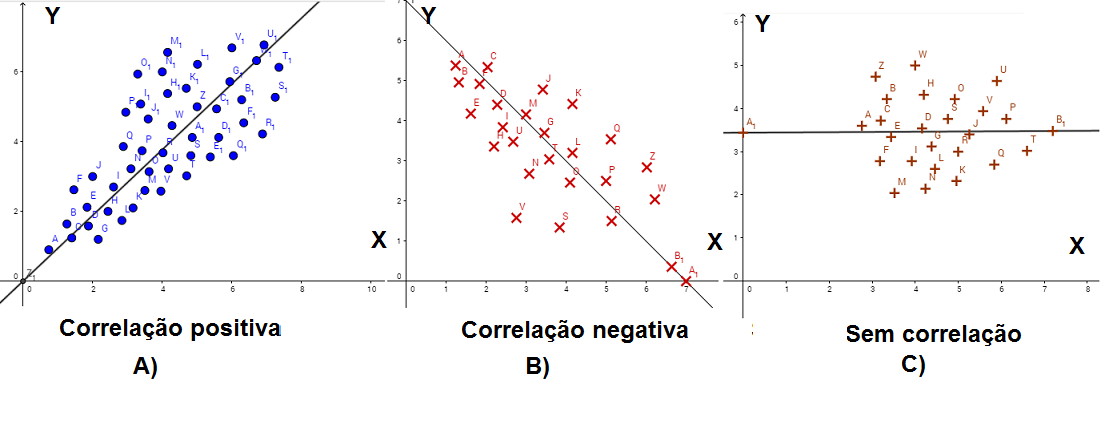
\includegraphics[width=\textwidth]{./Capitulo_3/correlacao_linha.png}	
	\caption{Figura demonstrando os tipos de correlação linear possíveis. A) Correlação linear positiva, B) Correlação linear negativa, C) Sem correlação }
	\label{correlacao_linear}
\end{figure}



Os gráficos de dispersão também são uma boa medida para a visualização de valores outliers. A figura \eqref{scatter_out} demonstra a dispersão anterior mas com uma área circulada de pontos que não estão dentro do comportamento linear das variáveis. Neste caso para valores intermediários de Cobalto temos grandes valores de Cromo.

 \begin{figure}[H]
 	\centering
 	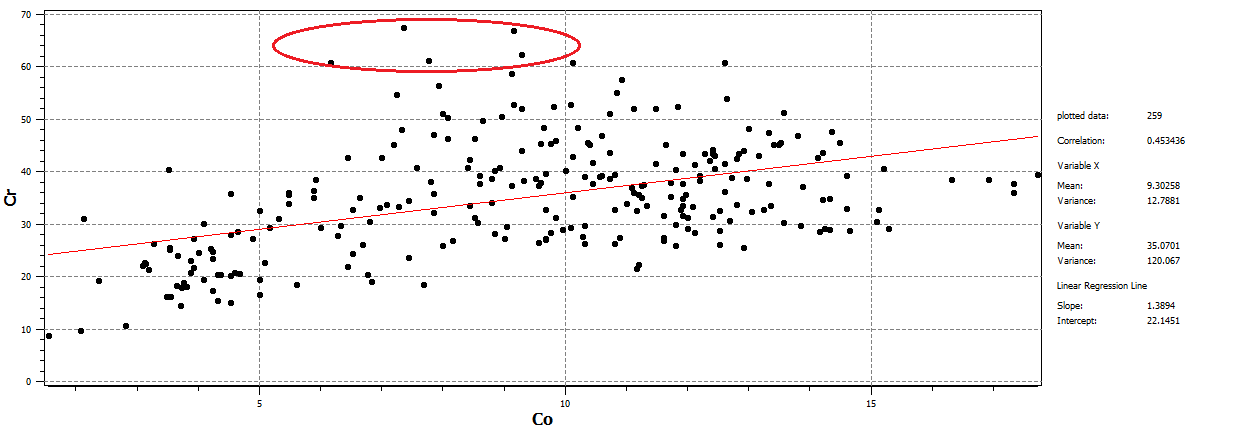
\includegraphics[width=\textwidth]{./Capitulo_3/scatter_out.png}	
 	\caption{Gráfico de dispersão da variável Cromo e Cobalto demonstrando valores outliers. Círculo vermelho indica possíveis valores fora dos padrões das variáveis conjuntas }
 	\label{scatter_out}
 \end{figure} 
 
 Muitas vezes um valor outlier em um gráfico bivariado não é demonstrado no tratamento individual das amostras. Muito cuidado deve ser tomado para a retirada de pares anômalos das estatísticas, pois eles podem gerar novos valores discrepantes e não demonstrarem um padrão de maior correlação entre as variáveis.
 
     
  \section{Regressão linear }
  
  O modelo de regressão linear simples é aquele em que definimos uma dependência diretamente proporcional entre a variável resposta Y e preditora X. Podemos associar o valor esperado da variável resposta dado valores da variável preditora tal que $E(Y|X=x) = \beta_{0} + \beta_{1}x$. Note que $E(Y|X=x)$ corresponde ao \textbf{valor médio da variável Y condicionado a um valor x da variável X}, e $\beta_{0}$ e $\beta_{1}$, também são o \textbf{intercepto da reta no eixo das abcissas} e \textbf{a tangente do ângulo de inclinação da reta}  . Muitas pessoas acabam por não entender que a regressão linear pode não apresentar uma representação acurada da resposta dado um valor da variável preditora, porque o valor estimado pela regressão não é o valor da variável resposta, mas sim seu valor esperado condicionado. Muitas variáveis apresentam alta dispersão em torno de seus valores médios e podem não ser estimativas plausíveis. a solução da \textbf{regressão linear ordinária} geralmente advém do método dos mínimos quadrados. Considere $\hat{y}_{i}=\hat{E}(Y|X=x)$ como um estimador para $E(Y|X=x)$, logo teremos que o resíduo pode ser demonstrado pela equação  $\hat{y}_{i}-y_{i}$ segundo a equação   
 
 \FloatBarrier 
 \begin{proof}
  	Regressão linear pelo método dos mínimos quadrados
  	\begin{align*}
  	&\epsilon_{i} =  \hat{y}_{i}-y_{i}  \\
  	&\epsilon_{i}^{2} = \hat{y}_{i}^{2} + y_{i}^{2} - 2\hat{y}_{i}y_{i}\\
  	&\epsilon_{i}^{2} = (\hat{\beta_{0}} + \hat{\beta_{1}}x_{i})^{2} + y_{i}^{2} - 2(\hat{\beta_{0}} + \hat{\beta_{1}}x_{i})y_{i}\\
  	&\text{A soma dos erros quadraticos para cada i} \\
  	&\sum_{i=0}^{n}\epsilon_{i}^{2} = \sum_{i=0}^{n}(\hat{\beta_{0}} + \hat{\beta_{1}}x_{i})^{2} + \sum_{i=0}^{n}y_{i}^{2} - \sum_{i=0}^{n}2(\hat{\beta_{0}} + \hat{\beta_{1}}x_{i})y_{i}\\
  	&\text{Tomando as derivadas parciais segundo os parâmetros: } \hat{\beta_{0}},\hat{\beta_{1}}\\
  	&1)\frac{\partial \sum_{i=0}^{n}\epsilon_{i}^{2}}{\partial \hat{\beta_{0}}} = 2\hat{\beta_{0}}n + 2\hat{\beta_{1}}\sum_{i=0}^{n}x_{i} - \sum_{i=0}^{n}2y_{i} = 0 \\
  	&2)\frac{\partial \sum_{i=0}^{n}\epsilon_{i}^{2}}{\partial \hat{\beta_{1}}} = 2\hat{\beta_{1}}\sum_{i=0}^{n}x_{i}^{2} + 2\sum_{i=0}^{n}\hat{\beta_{0}}x_{i} - 2\sum_{i=0}^{n}y_{i}x_{i} =0 \\
  	\end{align*}
  \end{proof}
 \FloatBarrier 
 
 
A obtenção dos parâmetros pode ser facilmente encontrada isolando os termos das equações 1 e 2. Podemos então determinar 

 \FloatBarrier 
\begin{proof}
 	Obtenção dos parâmetros da regressão
 	\begin{align*}
  	&\hat{\beta_{0}} = (\sum_{i=0}^{n}y_{i} - \hat{\beta_{1}}\sum_{i=0}^{n}x_{i})/n \\
  	&\text{Substituindo em 2}\\
  	&\hat{\beta_{1}}\sum_{i=0}^{n}x_{i}^{2} + \sum_{i=0}^{n}(\sum_{j=0}^{n}y_{j} - \hat{\beta_{1}}\sum_{j=0}^{n}x_{j})x_{i}/n - \sum_{i=0}^{n}y_{i}x_{i} =0 \\
  	&\hat{\beta_{1}}\sum_{i=0}^{n}x_{i}^{2} - \hat{\beta_{1}}\bar{x}\sum_{i=0}^{n}x_{i} + \bar{x}\sum_{i=0}^{n}y_{i} - \sum_{i=0}^{n}y_{i}x_{i} = 0  \\
  	&\hat{\beta_{1}}(\sum_{i=0}^{n}x_{i}^{2} - \bar{x}\sum_{j=0}^{n}x_{i}) = \sum_{i=0}^{n}y_{i}x_{i} - \sum_{j=0}^{n}y_{j}\bar{x}\\
  	&\hat{\beta_{1}} = \frac{\sum_{i=0}^{n}y_{i}x_{i} - \sum_{j=0}^{n}y_{j}\bar{x}}{\sum_{i=0}^{n}x_{i}^{2} - \bar{x}\sum_{j=0}^{n}x_{i}}\\
    \end{align*}
\end{proof}
 \FloatBarrier 
 
    
  O problema de regressão linear se torna então um problema de otimização ao encontrar o menor somatório dos desvios quadrádicos. A figura \eqref{scatter_expl} demonstra graficamente o problema da regressão linear. Neste caso os valores dos coeficientes lineares das retas podem ser encontrados a partir de derivação simples ou por meio de métodos numéricos, como a utilização do \textbf{método Simplex}. O resultado também é análogo ao \textbf{método de máxima verossimilhança} considerando a distribuição dos resíduos como gaussianos. 
  
\FloatBarrier  
\begin{figure}[!htbp]
  	\centering
  	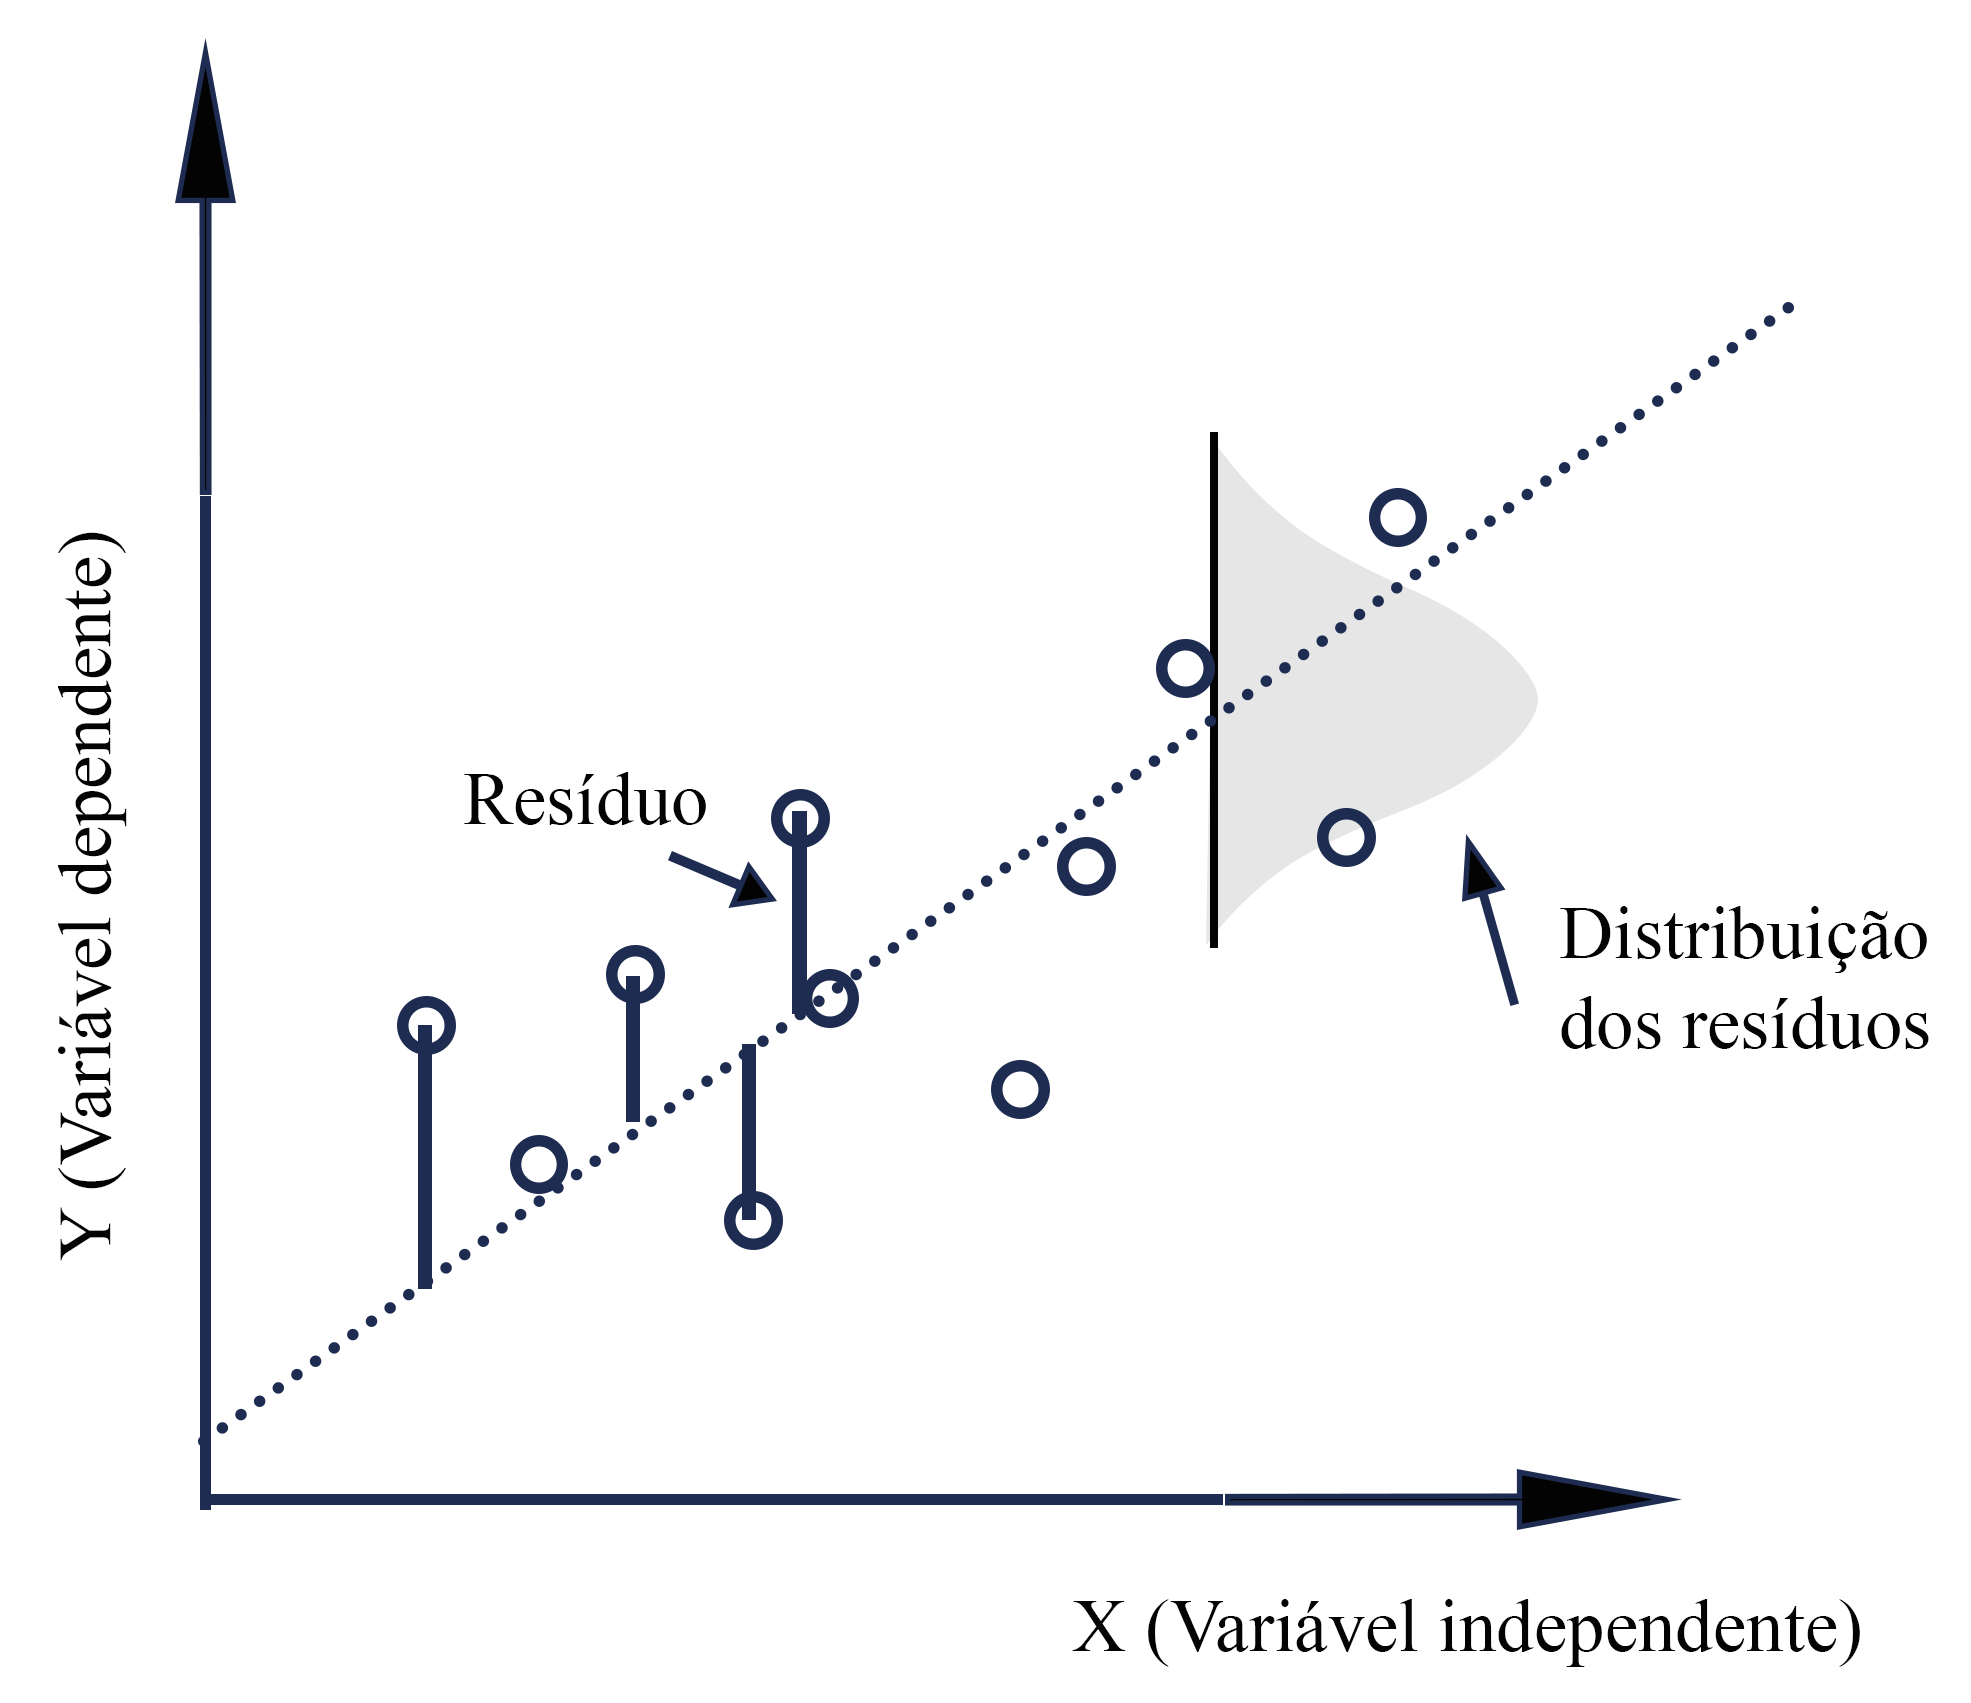
\includegraphics[scale=0.5]{./Capitulo_3/regress_expl.png}	
  	\caption{Explicação da regressão linear entre a variável independente X e a variável dependente Y. Barras verticais representando o os desvios das amostras com o valor médio. }
  	\label{scatter_expl}
\end{figure}
\FloatBarrier  

Como a regressão linear assume a minimização dos valores quadráticos, os parâmetros e $\beta_{0}$ e $\beta_{1}$ podem ser fortemente afetados por valores outliers. As propostas mais modernas de regressão prevem que a regressão seja utilizada apenas em parte dos dados, e avaliada com outra quantidade dos dados. Os dados utilizados para a estimativa dos parâmetros é chamada de  Assim conseguimos avaliar a qualidade da predição de acordo com a dispersão destes resíduos. 

\FloatBarrier
\begin{figure}[!htbp]
	\centering
	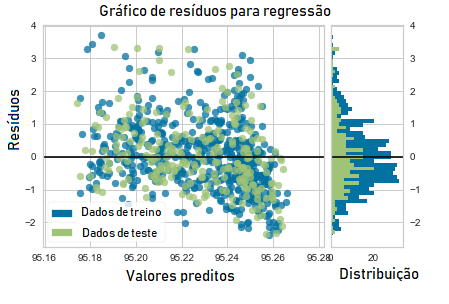
\includegraphics[scale=0.8]{./Capitulo_3/graf_resd.png}	
	\caption{Gráfico da dispersão de resíduos nos bancos de dados de treino e teste. Dados de treino utilizados para determinar os parâmetros da regressão e dados de teste para avaliar as diferenças do modelo de predição }
	\label{scatter_expl}
\end{figure}
\FloatBarrier
   
Na geoestatística utilizamos estimadores lineares, semelhantes ao processo de regressão linear. É observado que para aplicações na mineração  que utilizem os métodos geoestatísitcos clássicos, o erro do valor estimado é ligeiramente diferente de uma distribuição gaussiana, para problemas lineares e estacionários. Temos uma maior confiabilidade do valor esperado estimado utilizando krigagem ordinária do que utilizando regressão linear ordinária. Na verdade, o método de regressão linear ordinária é pouco usual nos dias atuais, considerando os diferentes modelos possíveis e robustos (menos influenciados pelos valores outliers), no entanto, ainda é um método muito popular pela sua simplicidade e facilidade de aplicação.

\begin{remark}
	\textit{Em aplicações da mineração, a distribuição dos erros da função aleatória são geralmente simétricos com um crescimento mais pronunciado na moda e caudas alongadas do que para distribuições normais com mesma média e variância. Então em relação a uma distribuição normal, há menos erros na região próxima ao valor esimado e mais erros nas caudas.} - \cite{journel1978mining}
\end{remark}
 
 \section{Intervalo de segurança para a regressão linear}
 
 A determinação do modelo de regressão consiste em estimar parâmetros $\beta_{0}$ e $\beta_{1}$ para econtrarmos o valor estimado $\hat{y}_{i} = E(Y|X=x_{i})$. No entanto, se a nuvem de pontos determinada pela regressão for esparsa, o valor $\hat{y}_{i}$ não possui capacidade preditiva e pode encontrar-se dentro de limites amplos. Considerando que a distribuição dos resíduos seja normalmente distribuída, podemos encontrar os limites da regressão para bandas superiores e inferiores, determinando assim a confiabilidade desta reta regredida.  A equação \eqref{intervalo_seguranca} demonstra como podem ser calculadas as bandas de incerteza da regressão de acordo com um nível de significância estipulado. 
 
 \begin{equation}\label{intervalo_seguranca}
	 \hat{y}_{i} \pm  t^{*}_{(n-2,p)} s_{y} \sqrt{\frac{1}{n}+\frac{(x_{i}-\bar{x})^2}{(n-1)s^2_{x}}}
 \end{equation}
 
 Em que $x_{i}$ é o valor da variável X, $t^*$ é o valor da distribuição de t-student para um grau de liberdade igual a $n-2$ e nível de significância p, enquanto $s_{y}$ pode ser demonstrado segundo a equação \eqref{intervalo_seguranca2}
 
  \begin{equation}\label{intervalo_seguranca2}
  s_{y} = \sqrt{\frac{\sum_{i}(y_{i}-\hat{y}_{i})^2}{n-2}}
  \end{equation}
   
  Em que $y_{i}$ é o valor da coordenada y para um ponto amostral i. Ou seja $s_{y}$ é o valor do desvio padrão entre os valores amostrais e os valores médios estimados pela regressão. 
  
  A figura \eqref{inter_seg} demonstra o intervalo de segurança para o valor regredido. 
  
  \begin{figure}[H]
  	\centering
  	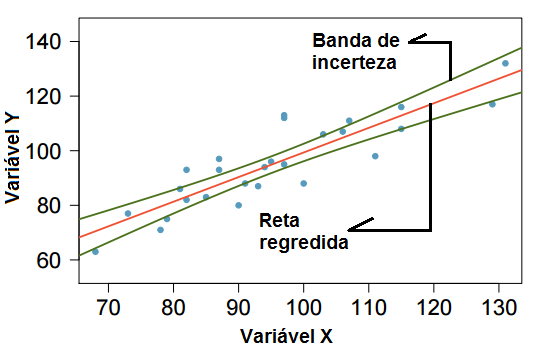
\includegraphics[scale=0.8]{./Capitulo_3/banda_incerteza.png}	
  	\caption{Demonstração do intervalo de confiança para a regressão linear. Banda de incerteza adicionada como limite inferior e superior dado pela equação \eqref{intervalo_seguranca} }
  	\label{inter_seg}
  \end{figure}
  
  Nota-se que as bandas apesar de acompanharem o valor de regressão linear não são retas, apresentado um maior estreitamento na região mediana da dispersão. A confiabilidade do centro de dispersão da reta regredida é sempre maior. 
  
 \begin{proposition}
 \textit{Os intervalos de confiança para a regressão linear estipulam que os resíduos seguem uma distribuição gaussiana. Isto porém, pode não se apresentar na prática. A única garantia que temos para que este resíduo seja considerado gaussiano, é se por ventura, a distribuição dos dados segue uma lei de probabilidades \textbf{multigaussiana}. Este é o pressuposto de técnicas mais avançadas de geoestatística não-linear. As bandas de incerteza devem ser consideradas como uma alternativa para verificar dados discrepantes, mas não como uma métrica de decisão na detecção de valores outliers.} 
 
\end{proposition}
  

  
 \section{Regressão linear múltipla}
 
 Quando pensamos em apenas uma variável preditora, a determinação de $\hat{y}_{i}$ se limita a encontrar o valor de $E(Y|X=x_{i})$. Porém quando múltiplas variáveis são relacionadas o problema se torna encontrar $E(Y|X^{1}=x^{1}_{i},X^{2}=x^{2}_{i},...,X^{n}=x^{n}_{i})$. O modelo de regressão linear múltipla é um caso extendido da regressão linear simples para múltiplas variáveis. Neste caso temos um conjunto de n variáveis preditoras e uma variável resposta
 
  \begin{equation}\label{eq1:Metodo_dos_minimos_quad}
  \hat{y}_{i} = \hat{\beta_{0}} + \hat{\beta_{1}} x^{1}_{i} + \hat{\beta_{2}} x^{2}_{i} + ... + \hat{\beta_{n}} x^{4}_{i} = \sum_{j=0}^{p} \hat{\beta_{j}} x^{j}_{i}
  \end{equation} 
  

  
  Onde $x^{0}_{i}$ é sempre igual a 1 para $j$ variáveis de 0 a p. O problema se resume a encontrar $\hat{\beta_{p}}$ parâmetros que aproximem melhor a combinação dos valores das variáveis $x^{p}_{i}$ de $\hat{y}_{i}$. Podemos definir o problema de regressão linear múltipla a partir de sua forma matricial pela equação \eqref{matricial}
  
  \begin{equation}\label{matricial}
  \begin{pmatrix}
  y_{1}\\ 
  y_{2}\\
  \vdots\\
  y_{n}
  \end{pmatrix}=\begin{pmatrix}
  1      & x^{1}_{1} & \cdots & x^{p}_{1}\\ 
  1      & x^{1}_{2} & \cdots & x^{p}_{2}\\ 
  \vdots & \vdots    & \vdots & \vdots \\ 
  1      & x^{1}_{n} & \cdots & x^{p}_{n}
  \end{pmatrix}\begin{pmatrix}
  \beta_{0}\\ 
  \beta_{1}\\
  \vdots\\
  \beta_{n}
  \end{pmatrix}
  \end{equation} 
  
  Ou de forma simplificada pela equação \eqref{matricial2}
  \begin{equation}\label{matricial2}
  	\bar{Y} = \bar{X}\bar{\beta}
  \end{equation}
  
  Onde $\bar{Y}$ representa o vetor da variável resposta, $\bar{X}$ a matriz das variáveis preditoras e $\bar{\beta}$ os parâmetros. A obtenção dos parâmetros a partir da regressão mútlipla pode ser facilmente encontrado através de operações matriciais.
  
 \FloatBarrier 
\begin{proof}
	Obtenção dos parâmetros da regressão
	\begin{align*}
	&\bar{Y} = \bar{X}\bar{\beta} \\
	&\bar{X}\bar{Y} = \bar{X}\bar{X}\bar{\beta} \\
	&(\bar{X}\bar{X})^{-1}\bar{X}\bar{Y} = \bar{\beta}\\
	&(\bar{X}\bar{X})^{-1}\bar{X}\bar{Y} = \bar{\beta}\\
	&X^{\dagger}\bar{Y}= \bar{\beta}\\
	&\text{tal que :} X^{\dagger} = (\bar{X}\bar{X})^{-1}X \\ 
	\end{align*}
\end{proof}
\FloatBarrier 
  
Em que $X^{\dagger}$ também é chamada de pseudo-inversa de X. Se no caso da regressão ordinária simples obtínhamos um valor regredido a partir da minimização do resíduo de uma variável, neste momento obtemos o resíduo a partir de uma combinação de múltiplas variáveis. O erro quadrático pode ser obtido a partir da equação \eqref{erroquad}. 
  
 
 \begin{equation}\label{erroquad}
 \sum_{i} \epsilon_{i}^2 = \sum_{i} \left( y_{i} - \sum_{j=0}^{p} \hat{\beta_{j}} x^{j}_{i} \right)^{2}
 \end{equation}
 
A obtenção dos parâmetros $\beta_{p}$ pode ser calculado a partir das técnicas de minimização dos resíduos, formando um sistema de $p$ derivadas parciais Um dos grandes problemas da regressão linear múltipla é o fato de que as grandezas de variáveis diversas podem ser diferentes e impactar de forma diferenciada nos pesos da regressão.Esse problema de dimensão geralmente pode ser minimizado se padronizarmos as variávies como visto no capítulo \ref{est_univ}. Outra questão envolvendo a regressão múltipla é o fato de que valores outliers conseguem ser ainda mais prejudiciais que a regressão linear ordinária, afetando muito a estimativa dos pesos. Uma tentativa de excluir certos efeitos de valores discrepantes é introduzir uma constante adicional chamada de \textbf{regularização} ($\lambda$) multiplicando os valores dos parâmetros $\beta_{p}$. 
  
  \section{Coeficiente de correlação }
  
  Observamos na seção anterior que se duas variáveis são dependentes, podemos assumir que existe uma probabilidade $P(Y|X=x)$. No entanto, as probabilidades condicionais parecem não fornecer um quadro geral da dependência de uma variável aleatória $Y$, pois precisamos saber qual valor a variável $X$ deve assumir. É necessário ter uma métrica para avaliarmos o quão forte ou fraca é a dependência entre as variáveis. Imagine o caso onde temos um depósito hidrotermal de ouro, associado principalmente a rochas magmáticas sulfetadas. Se existir uma alta dependência do conteúdo de ouro com o de enxofre, podemos assumir que o conhecimento de uma variável auxiliará no conhecimento da outra. Porém valores pequenos de teor de enxofre podem ser menos dependentes do teor de ouro do que para altos valores do teor de enxofre. Esta discrepância dado alguns limites pode ser favorável para o uso de probabilidades condicionais nas caudas da distribuição de enxofre, mas não garante uma visão geral da dependência linear entre estas variáveis. 
  
  \begin{remark}
  	\textit{Tanto na natureza como em vários problemas de engenharia nos deparamos com a dependência entre diferentes variáveis. Em muitos casos estas dependências podem ser modeladas linearmente. Em outros casos, quando conhecemos propriedades físicas relacionáveis, podemos utilizar \textbf{transformações lineares}, capazes de transformar modelos não lineares em lineares.} 
  \end{remark}

No capítulo \ref{cap_var_reg} observamos a correlação como uma medida de dependência entre variáveis aleatórias. A covariância teórica pode ser estimada a partir de sua covariância experimental pela equação \eqref{correst} 

\begin{equation}\label{correst}
\hat{Cov}_{X,Y} = \frac{\sum_{i=0}^{n} (x_{i} - \bar{x})(y_{i} - \bar{y})}{n}
\end{equation}

Onde $\bar{x}$ e $\bar{y}$ são as médias aritméticas entre as variáveis X e Y para um número de amostras n. A covariância experimental pode ser muito bem comparada ao produto escalar obtido pela multiplicação de dois vetores $X*Y = \left \| X\right \| \left \| Y  \right \| cos(\theta)$, em que $cos(\theta)$ é chamado de cosseno diretor da projeção de $X$ em $Y$. Quando a projeção do vetor $X$ corresponde ao vetor $Y$ temos o máximo valor possível, no entanto, quando estes vetores são perpendiculares temos um valor de $cos(90^{\circ})=0$, e portanto $\hat{Cov}_{X,Y} =0$  

A covariância é uma medida muito susceptível a valores outliers, pois como X e Y podem ter unidades discrepantes, o produto das duas pode ser mais influenciado por aquela variável que apresentar maiores valores. Imagine que procuremos a relação entre a massa em quilos dos testemunhos e o teor de um elemento químico. Como a massa dos testemunhos poderá variar de valores acima da unidade, como por exemplo 12kg e os teores apenas com valores decimais, como 0.12, a importância dada para as variações do peso serão maiores. Isto torna a a covariância pouco comparativa, apenas se considerarmos a normalização das variáveis. A alternativa para isto é normalizarmos a covariância pelos desvios padrões das respectivas variáveis, o que gera o \textbf{coeficiente de correlação de Pearson} \eqref{rozinho}.   


\begin{equation}\label{rozinho}
\rho_{X,Y}^{p} = \frac{\sum_{i=0}^{n} (x_{i} - \bar{x})(y_{i} - \bar{y})}{\sqrt{\sum_{i=0}^{n}(x_{i} - \bar{x})^{2}(y_{i} - \bar{y})^{2})}} 
\end{equation}
 
 Os valores de $\rho_{X,Y}$ podem variar de -1 a 1, sendo 1 quando apresenta correlação positiva perfeita e -1 quando apresenta correlação negativa perfeita. Quando $\rho_{X,Y}^{p} = 0$ temos um indicativo de independência entre as variáveis tal que $\hat{Cov}_{X,Y}$ é igual a 0. Podemos obter a relação entre o coeficiente de Pearson e a correlação pela equação \eqref{rozinho2}
 
 \begin{equation}\label{rozinho2}
 \rho_{X,Y}^{p} = \frac{\hat{Cov}_{X,Y}}{\sqrt{S_{x}^{2} S_{y}^{2}}} 
 \end{equation}
 
 Onde $\hat{Cov}_{X,Y}$ representa a covariância estimada, e $S_{x}^{2}$ e $S_{y}^{2}$ as variâncias experimentais das amostras x e y. Para que consigamos calcular o valor do coeficiente de variação e da correlação, precisamos que existam valores correspondentes tanto para as amostras x e y, ou seja, precisamos de dados \textbf{colocados}. Se por ventura houverem dados faltantes, não consiguiremos calcular a covariância ou o coeficiente de correlação. 
 
 Em alguns casos não desejamos observar a dependência entre os valores da variável, mas precisamos saber qual é a dependência da \textbf{ordem} dos dados. Para isto realizamos uma medida chamada de \textbf{rank ou posto}, que representa a ordem de uma amostra em seu conjunto. 
 
\begin{definition} [Rank ou posto]
	\textit{Um rank ou posto é a ordem crescente de uma amostra em seu respectivo conjunto. Por exemplo, um conjunto de amostras com valores $x={3,41,2,57,8,9,6}$, possuirá um rank $R_{x}$ tal qual $R_{x} = {2,6,1,7,4,5,3}$ }
\end{definition}
 
O chamado \textbf{coeficiente de correlação de Spearman} nada mais é que a correlação de Pearson considerando seus respectivos postos. 

 \begin{equation}\label{Spearman}
\rho_{X,Y}^{s} = \frac{\hat{Cov}_{R_{x},R_{y}}}{\sqrt{S_{R_{x}}^{2} S_{R_{y}}^{2}}} 
\end{equation}	 

Enquanto a correlação de Pearson é uma medida linear de dependência, o coeficiente de Spearman é uma medida não linear, demonstrando a correlação entre crescimentos e descrescimentos das variáveis independente dos valores dos dados. Uma função parabólica tal que $Y = \beta_{1} X^{2}  + \beta_{0} $ apresentará um valor de coeficiente de correlação de Pearson muito baixo, porém um valor de Coeficiente de Spearman igual a 1. 
\section{Exercícios}

\begin{exercise}
	
	Os dados da tabela abaixo representam valores de Au e cobre medidos concumitamente nos mesmos testemunhos de sondagem. Com estes dados, pede-se:
	
	a) Determine a covariância dos dados 
	
	b) Determine o coeficiente de correlação.
	
	c) As amostras são dependentes positivamente ou negativamente?
	
	d) Faça um gráfico de regressão linear entre as variáveis ouro e cobre
	
	\begin{tabular}{lllll}
		\hline
		Au & Cobre &  &  &  \\ \hline
		0.012      & 2.0  &  &  &  \\
		0.015      & 2.02 &  &  &  \\
		0.013      & 1.32 &  &  &  \\
		0.070      & 3.45 &  &  &  \\
		0.012      & 1.02 &  &  &  \\
		0.067      & 2.19 &  &  &  \\
		0.090      & 4.01 &  &  &  \\
		0.08      & 3.67 &  &  &  \\
		0.012      & 1.43 &  &  &  \\
		0.011      & 1.01 &  &  &  \\
		0.011      & 1.05 &  &  &  \\ \hline
	\end{tabular}
\end{exercise}

\begin{exercise}
	
	Os dados da tabela abaixo representam valores de X e Y. Faça um gráfico de dispersão e determine o par de valor outilier para o gráfico.
	
	\begin{tabular}{lllll}
		\hline
		X & Y &  &  &  \\ \hline
		0.729      & 1.546&  &  &  \\
		0.757      & 1.683&  &  &  \\
		0.140      & 0.175 &  &  &  \\
		0.575      & 0.963 &  &  &  \\
		0.408      & 0.726 &  &  &  \\
		0.402      & 1.104 &  &  &  \\
		0.616      & 1.321 &  &  &  \\
		0.958      & 5.02 &  &  &  \\
		0.9136      & 1.873 &  &  &  \\
		0.527      & 0.853 &  &  &  \\
		0.470      & 0.960 &  &  &  \\ \hline
	\end{tabular}
\end{exercise}